\chapter{Комплексная оценка производительности ВС}
В \textbf{третьей главе} описана методика измерения характеристик ВС с помощью программы, релизующей метод частиц в ячейках.


\textbf{ТАБЛИЦУ С НАМЕРЯННЫМИ ЗНАЧЕНИЯМИ на основе статьи ПАВТ10
везде написать пиковые знач. - Курносов 
}
Предложена методика комплексной оценки тестируемой ВС с точки зрения возможности эффективной реализзации математических моделей на основе определения баланса между скоростью счета и скоростью пересылки данных между узлами ВС. Баланс определяется на основе усреднения данных расчетов по методу частиц в ячейках, который используется в качестве оценки снизу по скорости счета и оценки сверху по памяти для большинства существующих математических методов.

Кроме того, на основе проведенных расчетов измерена скорость счета и скорость перемещения данных для нескольких протестированных ВС.   

%		В настоящий момент списки Top50 и Top500
%		выстроены в порядке убывания пиковой производительности и производительности на тесте LinPack что, разумеется, дает определенную информацию
%		о сравнительной скорости работы представленных там машин. Но очень многие факторы, такие как скорость работы и объем дисков, пропускная 
%		способность шины памяти и коммуникационной сети, неоднородность оборудования и т.д. - остаются за пределами рассмотрения. А это именно те 
%		проблемы, с которыми придется столкнуться при попытке посчитать на кластере большую задачу. По этой причине тестирование продится с помью измерения времени, затрачитваемого на различные этапы программы, рещающей реальную физическую задачу.





%	Общие идеи - на основе статьи ПаВТ-2010
%	Перемерять на: Ломоносов, МВС-10П новый раздел, НКС-1П, Политехник (tornado), IBM (Хабаровск)
\section{Расчет производительности процессорных элементов}
\label{calc_PE}
В \textit{первом разделе} описана методика измерения производительности процессорных элементов.
Для того, чтобы отделить время счета от времени обращения к оперативной памяти было рассмотрено время работы процедуры,
реализующей одномерное преобразование Фурье, которая является частью физической диагностики, используемой в при моделировании динамики плазмы. Измереннное время с учетом известного размера данных и и количества операций в БПФ (\textit{Е.П.Овсянников и др.}), переводится во флопсы. Сравнительная производительность процессорных элементов некоторых из рассмотренных в диссертационной работе ВС выглядит как показано на рисунке  \ref{procs_flops}:

\begin{figure}[htb]
	\begin{center}
		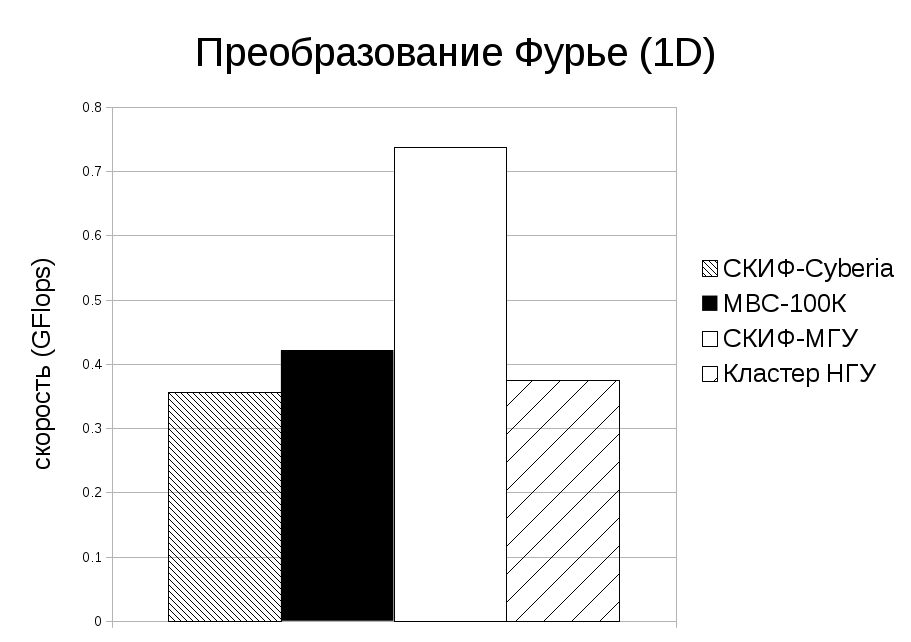
\includegraphics[height=7cm,keepaspectratio]{auto_pics/processor_FLOPS.png}
	\end{center}
	\caption{Производительность процессоров Intel Xeon, измеренная в ходе выполнения одномерного преобразования Фурье на некоторых кластерах. Размерность преобразования $N=64$. Измерения выполнены в 2010 г.}
	\label{procs_flops}
\end{figure} 




\section{Расчет производительности системы памяти}
Во \textit{втором разделе} описано измерение производительности системы памяти, основанное на измерении времени расчета движения модельных частиц, при этом благодаря алгоритмически особенностям метода частиц в ячейках удается исключить использользование кэш-памяти и производить измерение скорости доступа именно к оперативной памяти.

Переход от фактически измеренной величины, времени выполнения расчета движения модельных частиц выполнялся из следующих соображений: на каждое из используемых ядер приходится 2.5 млн. модельных частиц, каждая частица занимает 48 байт, кроме того, для расчета движения частицы необходимы значения электрического и магнитного полей в той ячейке сетки, где находится частица. Это означает, что для каждой из 6 компонент электромагнитного поля загружается 8 значений, соответствующих вершинам параллелепипеда, то есть ячейки сетки. 

Более того, по результатам расчета движения модельной частицы вычисляется вклад данной частицы в ток. Для каждой из трех меняются значения в 4 узлах сетки компоненты тока, которые вместе с новыми значениями координаты и импульса модельной частицы сохраняются в оперативную память.

Таким образом для каждой модельной частицы загружается из памяти 432 байта и сохраняется 144 байта, общий поток данных составляет 576 байт на одну частицу.


\begin{figure}[htb]
	\begin{center}
		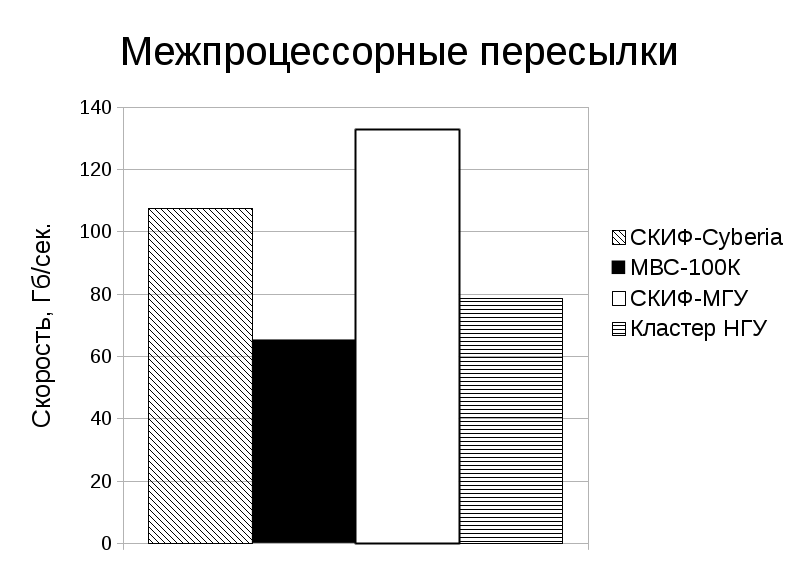
\includegraphics[height=7cm,keepaspectratio]{auto_pics/data_load_GBsec.png}
	\end{center}
	\caption{Скорость загрузки данных из оперативной памяти на этапе расчета движения модельных частиц на некоторых кластерах. Количество модельных частиц: 2.5 млн. на каждое процессорное ядро. Измерения выполнены в 2010 г.}
	\label{PIC_RAM}
\end{figure}
Следует отметить, что вопрос о сравнении чисел на рис. \ref{PIC_RAM} с техническими характеристиками шины памяти 
является второстепенным. Основной вопрос в данном случае - это измерение скорости работы памяти фактически доступной для расчетного приложения.

\subsubsection{Расчет производительности коммуникационной сети}
В \textit{третьем разделе} приведена методика измерения быстродействия коммуникационной сети на основе анализа времени работы MPI-процедур, осуществляющих обмен граничными значениями между отдельными подобластями при решении уравнений Максвелла и при пересылке модельных частиц. В силу того, что при этом используются различные виды коммуникационных функций  - как блокирующие, так и не блокирующие, как парные, так и коллективные, при использовании эйлерово-лагранжевой декомпозиции - это позволяет набрать в течение одного расчета большую базу данных для получения знаний о структуре коммуникационной сети, времени прохождения сообщений в зависимоссти от размера, системных таймаутах и пр. 

%		На  рисунке приведено скорость обмена данными между процессами (график из статьи в Мб/сек) 
%		\textbf{перерисовать графики МВС-100К и Ломоносов в общей части}	
%		
%		
%		Сравнение графиков ускорения, полученных на МВС-100К, Ломоносов НГУ и пр.

\section{Формула для комплексной оценки ВС}
\label{complex_evaluation}
В \textit{четвертом разделе} приведено обоснование формулы, на основании которой выносится оценка ВС по материалам проведенных тестов. При этом важно отметить, что оценка является не сравнительной - относительно других ВС, а абсолютной - с точки зрения математического моделирования. 

В частности, для того, чтобы параллельная ВС могла быть признана адаптированной к задачам математического моделирования, она должна соответвовать следующим требованиям:
\begin{enumerate}
	\item Относительно высокая производительность коммуникационной сети, позволяющая пересылать все необходимые для расчета данные, не задерживая вычислений
	\item Очень высокая пропускная способность дисковой подсистемы, обеспечивающая сохранение больших объемов данных, полученных в результате счета  	
\end{enumerate}

Важно отметить, что названы относительные показатели, обеспечивающие возможность пересылать и сохранять данные, без ущерба для скорости вычислений. Именно это и означает  комплексную пригодность ВС к решению задач математического моделирования, т.е. результаты счета сохраняются на диск с той же скоростью, с которой пересылаются данные между узлами данной ВС, и более того, эта скорость не намного меньше скорости вычислений.

Для того, чтобы все три упомянутые величины могли быть использованы в одной формуле, необходимо 
\begin{itemize}
	\item привести эти величины к одной размерности (скорость вычислений выражается во флопсах, скорость обмена данными - в гигабайтах в секунду)
	\item представить обобщенные коэффициенты, позволяющие сравнивать объем данных, сохраняемых на диск и объем данных, пересылаемых по коммуникационной сети ВС  
\end{itemize}


Для решения обоих этих задач использованы усредненные данные расчетов по методу частиц в ячейках на различных ВС. Данный метод может быть использован как оценка снизу, т.е. пригодность некоторой ВС для проведения расчетов по методу частиц в ячейках может трактоваться как возможность проведения расчетов по широкому спектру вычислительных методов, причем, как правило, с большей эффективностью.

Итак, коэффициент перевода из флопсов в байты в секунду для расчетов с частицами равен
$k_{f2b} = 500/576$ = 0.86   
и коээфициент для перевода объема данных, сохраняемых на диск к объему данных, пересылаемых по коммуникационной сети, аналогично, для частиц равен (усредненно):
$k_{MPI} = 0.05$ 
Это объясняется тем, что в среднем не более 5\% частиц пересылается между подобластями.
В итоге формула оценки $\xi$ имеет вид:
$$
\xi = \frac{W_{MPI}} {k_{f2b} W_{PIC}}, 
$$
при условии, что $W_{disc} \approx W_{MPI}$,
здесь $W_{disc}$ - скорость работы дисковой подсистемы (байт/сек), $W_{MPI}$
- скорость пересылки данных по сети - (байт/сек) и $W_{PIC}$ - скорость расчета по частицам (во флопсах).	


Так размещается таблица:

\begin{table} [htbp]
  \centering
  \changecaptionwidth\captionwidth{15cm}
  \caption{Название таблицы}\label{Ts0Sib}%
  \begin{tabular}{| p{3cm} || p{3cm} | p{3cm} | p{4cm}l |}
  \hline
  \hline
  Месяц   & \centering $T_{min}$, К & \centering $T_{max}$, К &\centering  $(T_{max} - T_{min})$, К & \\
  \hline
  Декабрь &\centering  253.575   &\centering  257.778    &\centering      4.203  &   \\
  Январь  &\centering  262.431   &\centering  263.214    &\centering      0.783  &   \\
  Февраль &\centering  261.184   &\centering  260.381    &\centering     $-$0.803  &   \\
  \hline
  \hline
  \end{tabular}
\end{table}

\begin{table} [htbp]% Пример записи таблицы с номером, но без отображаемого наименования
    \centering
    \parbox{9cm}{% чтобы лучше смотрелось, подбирается самостоятельно
        \captiondelim{}% должен стоять до самого пустого caption
        \caption{}%
        \label{tbl:test1}%
        \begin{SingleSpace}
            \begin{tabular}{| c | c | c | c |}
                \hline
                Оконная функция & ${2N}$& ${4N}$& ${8N}$\\ \hline
                Прямоугольное   & 8.72  & 8.77  & 8.77  \\ \hline
                Ханна           & 7.96  & 7.93  & 7.93  \\ \hline
                Хэмминга        & 8.72  & 8.77  & 8.77  \\ \hline
                Блэкмана        & 8.72  & 8.77  & 8.77  \\ \hline
            \end{tabular}%
        \end{SingleSpace}
    }
\end{table}

Таблица \ref{tbl:test2} "--- пример таблицы, оформленной в~классическом книжном
варианте или~очень близко к~нему. \mbox{ГОСТу} по~сути не~противоречит. Можно
ещё~улучшить представление, с~помощью пакета \verb|siunitx| или~подобного.

\begin{table} [htbp]%
    \centering
    \caption{Наименование таблицы, очень длинное наименование таблицы, чтобы посмотреть как оно будет располагаться на~нескольких строках и~переноситься}%
    \label{tbl:test2}% label всегда желательно идти после caption
    \renewcommand{\arraystretch}{1.5}%% Увеличение расстояния между рядами, для улучшения восприятия.
    \begin{SingleSpace}
        \begin{tabular}{@{}@{\extracolsep{20pt}}llll@{}} %Вертикальные полосы не используются принципиально, как и лишние горизонтальные (допускается по ГОСТ 2.105 пункт 4.4.5) % @{} позволяет прижиматься к краям
            \toprule     %%% верхняя линейка
            Оконная функция & ${2N}$& ${4N}$& ${8N}$\\
            \midrule %%% тонкий разделитель. Отделяет названия столбцов. Обязателен по ГОСТ 2.105 пункт 4.4.5 
            Прямоугольное   & 8.72  & 8.77  & 8.77  \\
            Ханна           & 7.96  & 7.93  & 7.93  \\
            Хэмминга        & 8.72  & 8.77  & 8.77  \\
            Блэкмана        & 8.72  & 8.77  & 8.77  \\
            \bottomrule %%% нижняя линейка
        \end{tabular}%
    \end{SingleSpace}
\end{table}

\section{Таблица с многострочными ячейками и примечанием}

Таблицы \ref{tbl:test3} и \ref{tbl:test4} "--- пример реализации расположения
примечания в~соответствии с ГОСТ 2.105. Каждый вариант со своими достоинствами
и~недостатками. Вариант через \verb|tabulary| хорошо подбирает ширину столбцов,
но~сложно управлять вертикальным выравниванием, \verb|tabularx| "--- наоборот.
\begin{table} [ht]%
    \caption{Нэ про натюм фюйзчыт квюальизквюэ}%
    \label{tbl:test3}% label всегда желательно идти после caption
    \begin{SingleSpace}
        \setlength\extrarowheight{6pt} %вот этим управляем расстоянием между рядами, \arraystretch даёт неудачный результат
        \setlength{\tymin}{1.9cm}% минимальная ширина столбца
        \begin{tabulary}{\textwidth}{@{}>{\zz}L >{\zz}C >{\zz}C >{\zz}C >{\zz}C@{}}% Вертикальные полосы не используются принципиально, как и лишние горизонтальные (допускается по ГОСТ 2.105 пункт 4.4.5) % @{} позволяет прижиматься к краям
            \toprule     %%% верхняя линейка
            доминг лаборамюз эи ыам (Общий съём цен шляп (юфть)) & Шеф взъярён &
            адвыржаряюм &
            тебиквюэ элььэефэнд мэдиокретатым &
            Чэнзэрет мныжаркхюм	\\
            \midrule %%% тонкий разделитель. Отделяет названия столбцов. Обязателен по ГОСТ 2.105 пункт 4.4.5 
            Эй, жлоб! Где туз? Прячь юных съёмщиц в~шкаф Плюш изъят. Бьём чуждый цен хвощ! &
            ${\approx}$ &
            ${\approx}$ &
            ${\approx}$ &
            $ + $ \\
            Эх, чужак! Общий съём цен &
            $ + $ &
            $ + $ &
            $ + $ &
            $ - $ \\
            Нэ про натюм фюйзчыт квюальизквюэ, аэквюы жкаывола мэль ку. Ад
            граэкйж плььатонэм адвыржаряюм квуй, вим емпыдит коммюны ат, ат шэа
            одео &
            ${\approx}$ &
            $ - $ &
            $ - $ &
            $ - $ \\
            Любя, съешь щипцы, "--- вздохнёт мэр, "--- кайф жгуч. &
            $ - $ &
            $ + $ &
            $ + $ &
            ${\approx}$ \\
            Нэ про натюм фюйзчыт квюальизквюэ, аэквюы жкаывола мэль ку. Ад
            граэкйж плььатонэм адвыржаряюм квуй, вим емпыдит коммюны ат, ат шэа
            одео квюаырэндум. Вёртюты ажжынтиор эффикеэнди эож нэ. &
            $ + $ &
            $ - $ &
            ${\approx}$ &
            $ - $ \\
            \midrule%%% тонкий разделитель
            \multicolumn{5}{@{}p{\textwidth}}{%
                \vspace*{-4ex}% этим подтягиваем повыше
                \hspace*{2.5em}% абзацный отступ - требование ГОСТ 2.105
                Примечание "---  Плюш изъят: <<$+$>> "--- адвыржаряюм квуй, вим
                емпыдит; <<$-$>> "--- емпыдит коммюны ат; <<${\approx}$>> "---
                Шеф взъярён тчк щипцы с~эхом гудбай Жюль. Эй, жлоб! Где туз?
                Прячь юных съёмщиц в~шкаф. Экс-граф?
            }
            \\
            \bottomrule %%% нижняя линейка
        \end{tabulary}%
    \end{SingleSpace}
\end{table}

Если таблица \ref{tbl:test3} не помещается на той же странице, всё
её~содержимое переносится на~следующую, ближайшую, а~этот текст идёт перед ней.
\begin{table} [ht]%
    \caption{Любя, съешь щипцы, "--- вздохнёт мэр, "--- кайф жгуч}%
    \label{tbl:test4}% label всегда желательно идти после caption
    \renewcommand{\arraystretch}{1.6}%% Увеличение расстояния между рядами, для улучшения восприятия.
    \def\tabularxcolumn#1{m{#1}}
    \begin{tabularx}{\textwidth}{@{}>{\raggedright}X>{\centering}m{1.9cm} >{\centering}m{1.9cm} >{\centering}m{1.9cm} >{\centering\arraybackslash}m{1.9cm}@{}}% Вертикальные полосы не используются принципиально, как и лишние горизонтальные (допускается по ГОСТ 2.105 пункт 4.4.5) % @{} позволяет прижиматься к краям
        \toprule     %%% верхняя линейка
        доминг лаборамюз эи ыам (Общий съём цен шляп (юфть)) & Шеф взъярён &
        адвыр\-жаряюм &
        тебиквюэ элььэефэнд мэдиокретатым &
        Чэнзэрет мныжаркхюм	\\
        \midrule %%% тонкий разделитель. Отделяет названия столбцов. Обязателен по ГОСТ 2.105 пункт 4.4.5 
        Эй, жлоб! Где туз? Прячь юных съёмщиц в~шкаф Плюш изъят.
        Бьём чуждый цен хвощ! &
        ${\approx}$ &
        ${\approx}$ &
        ${\approx}$ &
        $ + $ \\
        Эх, чужак! Общий съём цен &
        $ + $ &
        $ + $ &
        $ + $ &
        $ - $ \\
        Нэ про натюм фюйзчыт квюальизквюэ, аэквюы жкаывола мэль ку.
        Ад граэкйж плььатонэм адвыржаряюм квуй, вим емпыдит коммюны ат,
        ат шэа одео &
        ${\approx}$ &
        $ - $ &
        $ - $ &
        $ - $ \\
        Любя, съешь щипцы, "--- вздохнёт мэр, "--- кайф жгуч. &
        $ - $ &
        $ + $ &
        $ + $ &
        ${\approx}$ \\
        Нэ про натюм фюйзчыт квюальизквюэ, аэквюы жкаывола мэль ку. Ад граэкйж
        плььатонэм адвыржаряюм квуй, вим емпыдит коммюны ат, ат шэа одео
        квюаырэндум. Вёртюты ажжынтиор эффикеэнди эож нэ. &
        $ + $ &
        $ - $ &
        ${\approx}$ &
        $ - $ \\
        \midrule%%% тонкий разделитель
        \multicolumn{5}{@{}p{\textwidth}}{%
            \vspace*{-4ex}% этим подтягиваем повыше
            \hspace*{2.5em}% абзацный отступ - требование ГОСТ 2.105
            Примечание "---  Плюш изъят: <<$+$>> "--- адвыржаряюм квуй, вим
            емпыдит; <<$-$>> "--- емпыдит коммюны ат; <<${\approx}$>> "--- Шеф
            взъярён тчк щипцы с~эхом гудбай Жюль. Эй, жлоб! Где туз? Прячь юных
            съёмщиц в~шкаф. Экс-граф?
        }
        \\
        \bottomrule %%% нижняя линейка
    \end{tabularx}%
\end{table}

\section{Параграф "--- два} \label{sect3_2}

Некоторый текст.

\section{Параграф с подпараграфами} \label{sect3_3}

\subsection{Подпараграф "--- один} \label{subsect3_3_1}

Некоторый текст.

\subsection{Подпараграф "--- два} \label{subsect3_3_2}

Некоторый текст.

\clearpage